\documentclass[a4paper,11pt]{article}
\usepackage[T1]{fontenc}
\usepackage[utf8]{inputenc}
\usepackage{lmodern}
\usepackage{amsmath}
\usepackage{amsfonts}
\usepackage{amssymb}
\usepackage{amsthm}
\usepackage{graphicx}
\usepackage{color}
\usepackage{url}
\usepackage{textcomp}
\DeclareMathOperator*{\argmax}{argmax}
\DeclareMathOperator*{\argmin}{argmin}

\title{Value Iteration}
\author{Joshua Tsang}
\date{\today}

\begin{document}

\maketitle
\tableofcontents

\section{Foundational Concepts}

It is instructive intially discuss the foundational concepts in Markov Decision Problems (MDP) and Reinforcement Learning (RL).  Consider the problem shown in Figure \ref{fig:1d-grid-world-problem-statement} where an agent is located in one of the grid positions.

\begin{figure}
    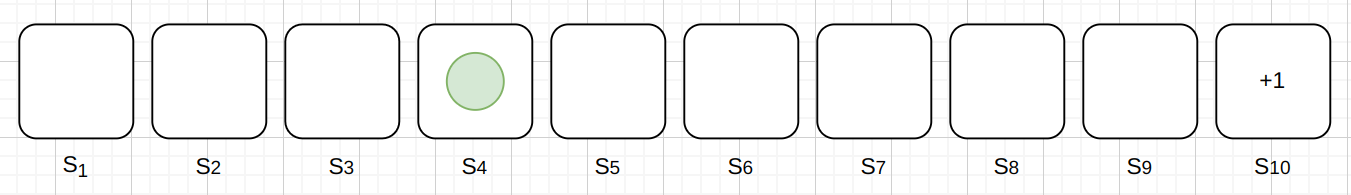
\includegraphics[width=\textwidth]{images/1d-grid-world-problem-statement.png}
    \caption{1D Grid World MDP with an assigned reward of $+10$ in state $s_{10}$, termed the terminal state.  The agent currently sits in state $s_4$ and the goal of the problem is for the agent to take actions to maximise its reward.  At each state other than the terminal state, there is a negative reward of $-1$.  Drawn with draw.io and saved in Google Drive as 1D\_grid\_world.drawio.}
    \label{fig:1d-grid-world-problem-statement}
\end{figure}


\begin{itemize}
    \item State Space and State: The finite State Space of a system is denoted $S$ where a state $s$ denotes a certain configuration of the system i.e. $s \in S$.  For example, in Figure \ref{fig:1d-grid-world-problem-statement} the agent is currently in state $s_4$, with the neighbouring states, $\{s'\}$, being $s_3$ and $s_5$.
    \item Actions: For each state, $s_i$, that the system resides in a set of available actions, $\{a_k\}$, can be taken that transition the system to another state, $s_j$.  For Figure \ref{fig:1d-grid-world-problem-statement} the available actions at state $s_4$ are \verb|(move left)| and \verb|(move right)|.  One could think of a graph where nodes are states and the edges are actions.
    \item Policy: A policy, denoted $\pi$, is a distribution over actions given states.  It is often written as a function $\pi(a|s)$ or $\pi(s, a)$ where it is formally defined as:
    \begin{equation} \label{eqn:policy_formal_definition}
        \pi(a|s) = \pi(s,a) = P(A_t=a|S_t=s)
    \end{equation}
    which is the probability of taking action $a$ given the system is in state $s$ at time step $t$. As such, $\pi(s, a)$ returns a probability value in the range $[0,1]$. The goal of RL is to learn the optimal policy $\pi(s,a)$ to maximise future rewards/returns (explained next). As a foreshadow, {\it optimal} policy functions are often expressed as an $\argmax_a$ as follows:
    \begin{equation} \label{eqn:value_iteration_foreshadow}
    \begin{split}
        \pi_{*}(s,a) &= \argmax_a \sum_{s'} \sum_{r} P(s',r|s,a)[r + \gamma v_{\pi}(s')] \\
        &= \argmax_a q_{*} (s,a)
    \end{split}
    \end{equation}
    i.e. the optimal policy function returns the action $a$ that transitions the agent to the neighbouring state $s'$ that yields the maximum transition-probability-weighted sum of the returns, or in other words, the maximum {\it action value} as discussed around equation (\ref{eqn:action_value_function_definition}).
    \item Reward: Numerical reward can be associated with certain states and actions, represented as $R_t$ for the current time step.  In the case of Figure \ref{fig:1d-grid-world-problem-statement}, there is a fixed reward of $+10$ at state $s_{10}$ and the other states have a reward of $-1$.  The goal of RL can be considered to be finding the sequence of actions that maximise the sum of rewards to achieve a sucessful episode i.e. the agent reaches the terminal state $s_{10}$.
    \item Episodes:  MDPs have the characteristic of being finite i.e. they end within a finite number of time steps, denoted $T$.  More specifically, an episode is a sequence of states, actions and rewards that start at some state and end in the terminal state.
    \item Return or "Future Gains":  Usually denoted $G_t$ it is the sum of rewards gained by the agent {\it after} time step $t$, define as:
    \begin{equation} \label{eqn:return_G_t}
        G_t = R_{t+1} + R_{t+2} + ... + R_{T}
    \end{equation}
    Before going further, it's worth appreciating how important this concept is to the definition of state value functions, $v(s)$, which try to capture the expected rewards to be gained by being in that state, $s$.

    It is possible to introduce a discount rate $\gamma \in [0,1]$ that diminishes the rewards gained further in the future:
    \begin{equation} \label{eqn:return_G_t_discounted}
    \begin{split}
        G_t &= R_{t+1} + \gamma R_{t+2} + \gamma^2 R_{t+3} + ... + \gamma^{T-1-t} R_{T} \\
        &= \sum_{k=t+1}^{T} \gamma^{k-1-t}R_k
    \end{split}
    \end{equation}
    note how the power of $\gamma$ in the final term is $T-1-t$ and {\it not} $T$, a little thought makes this clear (for example, try write down $G_4$ where $T=8$).  Finally, we note that the discounted expression can be rewritten into a recursive expression somewhat similar to Bellman's equation:
    \begin{equation} \label{eqn:return_G_t_like_bellmans_eqn}
    \begin{split}
        G_t &= R_{t+1} + \gamma R_{t+2} + \gamma^2 R_{t+3} + ... + \gamma^{T-1-t} R_{T} \\
        &= R_{t+1} + \gamma( R_{t+2} + \gamma R_{t+3} + ... + \gamma^{T-t} R_{T}) \\
        &= R_{t+1} + \gamma G_{t+1}
    \end{split}
    \end{equation}
    Expression (\ref{eqn:return_G_t_like_bellmans_eqn}) links the current return, $G_t$, to the return at the next time step, $G_{t+1}$.
\end{itemize}

\subsection{Markov Reward Process vs Markov Decision Process}

It is instructive to discuss Markov Reward Process (MRP) which are simpler than a Markov Decision Process (MDP).  This discussion helps consolidate concepts surrounding transition probabilites, policies and action values.  In short, an MDP is essentially an MRP {\it with actions} and thus an MRP will still have states, rewards and transition probabilties.  The transition probabilities encapsulate the dynamics of the process or the effects of the environment.  

Consider the MRP shown in Figure \ref{fig:slippery-world-mrp} which describes a `slippery world' MRP where the transition probabilities of moving to adjacent states is only succesful with probability 0.8, with a 0.2 chance of remaining in the same state.

\begin{figure}
    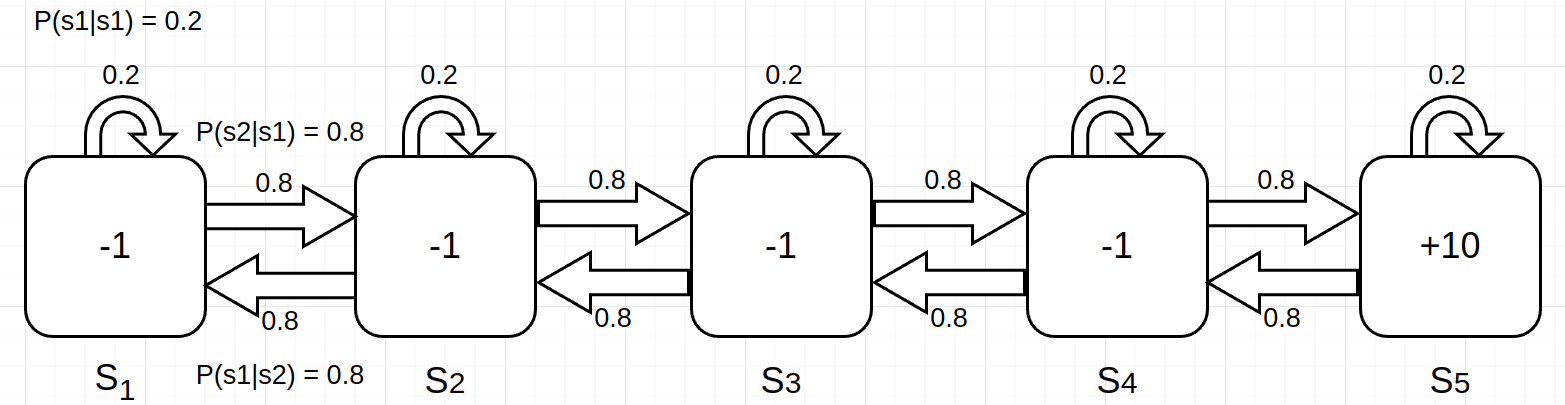
\includegraphics[width=\textwidth]{images/slippery_world_mrp.png}
    \caption{The Slippery World MRP where there's a 0.2 chance of remaining in the present state as the agent can slip and fall, making no movement progress.  There are still rewards associated with the states, hence the name Markov {\it Reward} Process.  Drawn with draw.io and saved in Google Drive.}
    \label{fig:slippery-world-mrp}
\end{figure}

The state transition matrix, ${\bf P}$, for the MRP can be written:
\begin{equation} \label{eqn:state_transition_matrix_for_slippery_world}
\begin{split}
        {\bf P} &=  
        \begin{pmatrix}
        P(s_1|s_1) & P(s_2|s_1) & P(s_3|s_1) & \hdots & P(s_N|s_1) \\
        P(s_1|s_2) & P(s_2|s_2) & P(s_3|s_2) & \hdots & P(s_N|s_2) \\
        \vdots & \vdots & \vdots & \ddots & \vdots \\
        P(s_1|s_N) & P(s_2|s_N) & P(s_3|s_N) & \hdots & P(s_N|s_N)
        \end{pmatrix} \\
        &= 
        \begin{pmatrix}
        0.2 & 0.8 & 0.0 & 0.0 & 0.0 \\
        0.8 & 0.2 & 0.8 & 0.0 & 0.0 \\
        0.0 & 0.8 & 0.2 & 0.8 & 0.0 \\
        0.0 & 0.0 & 0.8 & 0.2 & 0.8 \\
        0.0 & 0.0 & 0.0 & 0.8 & 0.2 
        \end{pmatrix}
\end{split}
\end{equation}

Knowing these state transition probabilties allows trajectories to be sampled and expect returns to be calculated.  Like an MDP, state values for each state, $v(s)$, can be computed.  In fact, the state values can be computed analytically using the linear equation:
\begin{equation} \label{eqn:linear_eqn_for_mrp}
\begin{split}
        \begin{pmatrix}
            v(s_1) \\
            v(s_2) \\
            \vdots \\
            v(s_5)
        \end{pmatrix} &=
        \begin{pmatrix}
            r(s_1) \\
            r(s_2) \\
            \vdots \\
            r(s_5)
        \end{pmatrix} +
        \gamma 
        \begin{pmatrix}
            P(s_1|s_1) & P(s_2|s_1) & P(s_3|s_1) & \hdots & P(s_5|s_1) \\
            P(s_1|s_2) & P(s_2|s_2) & P(s_3|s_2) & \hdots & P(s_5|s_2) \\
            \vdots & \vdots & \vdots & \ddots & \vdots \\
            P(s_1|s_5) & P(s_2|s_5) & P(s_3|s_5) & \hdots & P(s_5|s_5)
        \end{pmatrix}
        \begin{pmatrix}
            v(s_1) \\
            v(s_2) \\
            \vdots \\
            v(s_5)
        \end{pmatrix} 
        \\
        {\bf v} &= {\bf r} + \gamma {\bf P} {\bf v} 
\end{split}
\end{equation}
which allows the state values to be solved using some linear algebra as:
\begin{equation} \label{eqn:inverse_of_linear_eqn_for_mrp}
\begin{split}
    {\bf v} = ({\bf I} - \gamma {\bf P})^{-1} {\bf r}
\end{split}
\end{equation}
Solving the matrix is roughly $O(N^3)$ where $N$ is the number of states.



\section{Playing with Episodes of an MDP}

Recall that epsiodes are a sequence of states, actions and rewards that end in the terminal state.  Each episode yields a return/gain at $T$, which is $G_T$.  To clarify concepts and develop some intuitive, consider a few episodes for the Grid World system in Figure \ref{fig:1d-grid-world-problem-statement}.  The actions are $a \in [\text{LEFT}, \text{RIGHT}]$

\begin{itemize}
  \item Episode Example 1:
  
  $[S_{t=1} = s_4, A_{t=1} = \text{RIGHT}, G_{t=1}=-1]$ \\
  $[S_{t=2} = s_5, A_{t=2} = \text{RIGHT}, G_{t=2}=-2]$ \\
  $[S_{t=3} = s_6, A_{t=3} = \text{RIGHT}, G_{t=3}=-3]$ \\
  $[S_{t=4} = s_7, A_{t=4} = \text{RIGHT}, G_{t=4}=-4]$ \\
  $[S_{t=5} = s_8, A_{t=5} = \text{RIGHT}, G_{t=5}=-5]$ \\
  $[S_{t=6} = s_9, A_{t=6} = \text{RIGHT}, G_{t=6}=-6]$ \\
  $[S_{t=7} = s_10, A_{t=7} = \text{RIGHT}, G_{t=7}=+4]$ \\

  Note that this episode yields $G_T = +4$.

  \item Episode Example 2:
  
  $[S_{t=1} = s_4, A_{t=1} = \text{RIGHT}, G_{t=1}=-1]$ \\
  $[S_{t=2} = s_5, A_{t=2} = \text{RIGHT}, G_{t=2}=-2]$ \\
  $[S_{t=3} = s_6, A_{t=3} = \text{RIGHT}, G_{t=3}=-3]$ \\
  $[S_{t=4} = s_7, A_{t=4} = \text{RIGHT}, G_{t=4}=-4]$ \\
  $[S_{t=5} = s_8, A_{t=5} = \text{LEFT}, G_{t=5}=-5]$ \\
  $[S_{t=6} = s_7, A_{t=6} = \text{RIGHT}, G_{t=6}=-6]$ \\
  $[S_{t=7} = s_8, A_{t=7} = \text{RIGHT}, G_{t=7}=-7]$ \\
  $[S_{t=8} = s_9, A_{t=8} = \text{RIGHT}, G_{t=8}=-8]$ \\
  $[S_{t=9} = s_10, A_{t=9} = \text{RIGHT}, G_{t=9}=+2]$ \\
  
  Note that this episode yields $G_T = +2$, it is lower than Episode Example 1 because at $t=5$ it backtracks by going LEFT which caused it to require a longer path, and thus suffer more from the $R_t = -1$ penalties for the non-terminal states.
\end{itemize}

\section{State Value Function and Bellman's Equation}

An important concept in RL is the state value function, $v_{\pi}(s)$, which captures the expected return from being in state $s$.  It is critical to realise that the subscript $\pi$ in $v_{\pi}(s)$ means it must be evaluated for a given policy $\pi(a|s)$ since $v_{\pi}(s)$ is an expectation value (read: average) of potential returns by being in state $s$, which in turn depends on the expected return from the neighbouring states, $v_{\pi}(s')$.  In fact, this is why the Bellman equation in equation (\ref{eqn:bellmans_equation_part3}) has $v_{\pi}(s)$ on the LHS and $v_{\pi}(s')$'s on the RHS.

Since the policy $\pi(a|s)$ encapsulates the current policy's probability of taking action $a$ given the current state is $s$ (recall equation \ref{eqn:policy_formal_definition}), it thus influences the expected returns of being in the current state $s$.  In fact, it's prudent to think of the state value function as a function that ultimately links the state values of all states together.

The state value function, $v_{\pi}(s)$ of an MDP is the expected return starting from state $s$ and following the policy $\pi$:
\begin{equation} \label{eqn:bellmans_equation_part1}
\begin{split}
        v_\pi (s) &= \mathbb{E}[G_t|s] \\
        &= \sum_{a} \pi(a|s) \mathbb{E} [G_t|s,a]
\end{split}
\end{equation}
This is fairly intuitive, the state value is equal to the sum of the expected returns from all available actions $a$ at state $s$ weighted by the present policy probability distribution, $\pi$.

Using Equation (\ref{eqn:return_G_t_like_bellmans_eqn}) we can rewrite $\mathbb{E} [G_t|s, a]$ as:
\begin{equation} \label{eqn:bellmans_equation_part2}
\begin{split}
        \mathbb{E} [G_t|s, a] &= \mathbb{E} [R_{t+1} + \gamma G_{t+1}|s, a] \\
        &= \mathbb{E} [R_{t+1} + \gamma v_\pi(S_{t+1})|s, a] \\
        &= \sum_{s'} \sum_r P(s',r|s,a) [r + \gamma v_{\pi}(s')]
\end{split}
\end{equation}

This is in fact the action value function as discussed in the next section.  The final expression after substitution back into equation (\ref{eqn:bellmans_equation_part1}) is:
\begin{equation} \label{eqn:bellmans_equation_part3}
\begin{split}
        v_\pi (s) &= \sum_{a} \pi(a|s) \sum_{s'} \sum_r P(s',r|s,a) [r + \gamma v_{\pi}(s')]
\end{split}
\end{equation}
Equation (\ref{eqn:bellmans_equation_part3}) allows us to calculate the expected return value for each state in the MDP given the current policy, $\pi$, which may not yet be optimal.  We haven't yet discussed optimal policies at all and equation (\ref{eqn:bellmans_equation_part3}) simply calculates state values for a given policy $\pi(a|s)$.  It is the goal of RL to find the optimal policy, $\pi_*$, via methods like General Policy Iteration (GPI), Policy Iteration or Value Iteration to discover optimal policies.

Note that the probabilities $P(s',r|s,a)$ are not to be confused with the policy $\pi(s,a)$ but are transition probabilities intrinsic to the MDP that capture the dynamics of the environment.  Note that for an MRP the state transition probabilties are merely $P(s'|s)$ while for an MDP (which includes actions) it is $P(s',r|s,a)$ which encapsulates probabilties to transition into $s'$ for a given action $a$.  For instance, we could introduce a strong fan effect that blows left in state $s_4$ of the MDP in Figure \ref{fig:1d-grid-world-problem-statement} where there's now a 0.2 chance of the agent losing its footing/grip and will be blown back to state $s_3$.  These envionmental dynamics/effects are captured in the transition probabilities of the MDP.  So in this case, if we're in state $s_4$ then $P(s_5,r|s_4, a=\text{RIGHT}) = 0.8$ and $P(s_3,r|s_4, a=\text{RIGHT}) = 0.2$ i.e. there's a 0.2 chance of transitioning into the state in the opposite direction.  The goal of RL is to deduce the optimal policy taking into account these environmental/dynamic effects.

Now is a good time to mention model-based and model-free processes.  A model-based process has full knowledge of the transition probabilities $P(s',r|s,a)$, which although introduce a probabalistic element to the process, these transitions are known and the MDP is well-defined.  

(Talk about Gambler's problem and the transition probabilities in that.)


\subsection{Evaluating the state value function for an example MDP}

Consider the `Slippery World' MRP shown in Figure \ref{fig:slippery-world-mrp} and consider that we promote it to an MDP complete with actions.  At each state, there are 2 actions $a \in \{a_1, a_2\}$ where $a_1$ and $a_2$ represent the actions move LEFT and move RIGHT respectively.  Since the MDP has $S = 5$ states and each state has $A = 2$ actions, the total number of possible policies is $A^S = 2^5 = 32$.  Each state only has one `good' action so one can imagine each policy being like a binary sequence: $01110$ for example means $[a_1,a_2,a_2,a_2,a_1]$ and it's easy to imagine there are 32 possible combinations of these actions.

Let's try and evaluate the state value function equation (\ref{eqn:bellmans_equation_part3}) for state $s_4$ given the policy defined as follows:
\begin{equation} \label{eqn:example_policy_for_slippery_world}
\begin{split}
\begin{bmatrix}
    (\pi(a_1|s_1),\pi(a_2|s_1)) \\
    (\pi(a_1|s_2),\pi(a_2|s_2)) \\
    (\pi(a_1|s_3),\pi(a_2|s_3)) \\
    (\pi(a_1|s_4),\pi(a_2|s_4)) \\
    (\pi(a_1|s_5),\pi(a_2|s_5)) 
\end{bmatrix} &= 
\begin{bmatrix}
    (0.4, 0.6) \\
    (0.4, 0.6) \\
    (0.4, 0.6) \\
    (0.4, 0.6) \\
    (0.4, 0.6) 
\end{bmatrix}
\end{split}
\end{equation}
So the policy here is a 0.4 and 0.6 chance of taking action to move LEFT and RIGHT respectively, it effectively tries to do a 40/60 random walk in this slippery world but note it might not be able to actually do a perfect random walk due to the slippery dynamics encoded into the transition probabilities $P(s',r|s,a)$.  Computing $v_{\pi}(s_4)$ with a discount factor of $\gamma=0.5$:
\begin{equation} \label{eqn:v_s4_for_slippery_world}
\begin{split}
    v_{\pi}(s_4) &= \pi(a_1|s_4) [
        P(s_4,r|s_4,a_1)(r + \gamma v_{\pi}(s_4)) +
        P(s_3,r|s_3,a_1)(r + \gamma v_{\pi}(s_3))
    ] \\
    &+ \pi(a_2|s_4) [
        P(s_4,r|s_4,a_2)(r + \gamma v_{\pi}(s_4)) +
        P(s_5,r|s_4,a_2)(r + \gamma v_{\pi}(s_5))
    ] \\
    &= 0.4 [ 0.2 (-1 + 0.5 \times -1) + 0.8 (-1 + 0.5 \times -1) ] \\
    &+ 0.6 [ 0.2 (-1 + 0.5 \times -1) + 0.8 (+10 + 0.5 \times +10) ] \\
    &= -0.36 + 7.38 \\
    &= 7.02
\end{split}
\end{equation}
A similar computation can be performed for all states in the MDP.  Note that a different policy $\pi$ would give a different value for $v_{\pi}(s_4)$.  For example, if $\pi(a_1|s_4) = 1.0$ and $\pi(a_2|s_4) = 0.0$ then none of $s_5$'s significant +10 reward will be included in the value of $v_{\pi}(s_4)$ yielding a much lower state value.  It is clear that for each state, there exists a policy that would maximise their state values.  For $s_4$ it is clear to let $\pi(a_1|s_4) = 0.0$ and $\pi(a_2|s_4) = 1.0$ so the agent always tries to move RIGHT to claim that significant +10 reward.  

Note what might happen through repeated applications/sweeps of equation (\ref{eqn:bellmans_equation_part3}) to all the states of the MDP.  It intuitive to see that the fixed +10 reward in state $s_5$ will gradually `trickle' down into the state values of the states on the left.  



\section{State-Action Value Function, Q-Value Tables and Optimal Policies}

The action value function, denoted $q_{\pi}$, is defined as the inner sums in Equation (\ref{eqn:bellmans_equation_part3}):
\begin{equation} \label{eqn:action_value_function_definition}
    q_{\pi}(s,a) = \sum_{s'} \sum_r P(s',r|s,a) [r + \gamma v_{\pi}(s')]
\end{equation}
where $s'$ are the neighbouring states to the current state, $s$.  Do not confuse state values functions and state-action value functions.  State-action value functions include the action in the argument, naturally!  Equation (\ref{eqn:action_value_function_definition}) allows the optimal policy, $\pi_{*}$, to be written succinctly as:
\begin{equation} \label{eqn:optimal_policy_wrt_action_values}
    \pi_{*}(s) = \argmax_a q_{\pi}(s,a)
\end{equation}
You will notice that `optimal' expressions usually have some form of $\max_s$ or $\argmax_a$ in it.

It is instructive to represent Equation (\ref{eqn:action_value_function_definition}) computed as a matrix for a particular MDP in the following manner:
\begin{equation} \label{eqn:q-value-table}
\begin{bmatrix}
    q(s_1,a_1) & q(s_1,a_2) & \hdots & q(s_1,a_K) \\
    q(s_2,a_1) & q(s_2,a_2) & \hdots & q(s_2,a_K) \\
    \vdots & \vdots & \ddots & \vdots \\
    q(s_N,a_1) & q(s_N,a_2) & \hdots & q(s_N,a_K)
\end{bmatrix}
\end{equation}
where $N$ is the number of states and $K$ is the number of actions per state.  Matrix (\ref{eqn:q-value-table}) is often referred to as a `Q-value table'.  

As a foreshadow, Q-Learning attempts to construct this Q-value table which is used by the agent to determine the optimal action for a given state by selecting the action that yields the maximum $q$ value.  So say for $s_4$ in the Slippery World MDP, the agent will look at the row for $s_4$ and pick the action $a$ (column) that yields the greatest $q(s_4, a)$ value.  You may wonder how to compute the Q-value table if we don't know the optimal policy.  The exact details of how the Q-value table is constructed will not be explicitly stated here, but note that Q-Learning is an {\it off-policy} learning scheme and thus exploration of the state space is done by a behaviour policy, $b(a|s)$, instead of $\pi(a|s)$ in the case of on-policy schemes.



\section{Value Iteration}

Value iteration allows one to assign state values to each state through repeated, iterative application of the value function, and the optimal policy is extracted at the end.  

Look at 1:08:23 in Lecture 2 of Stanford RL Youtube video.


\begin{figure}
    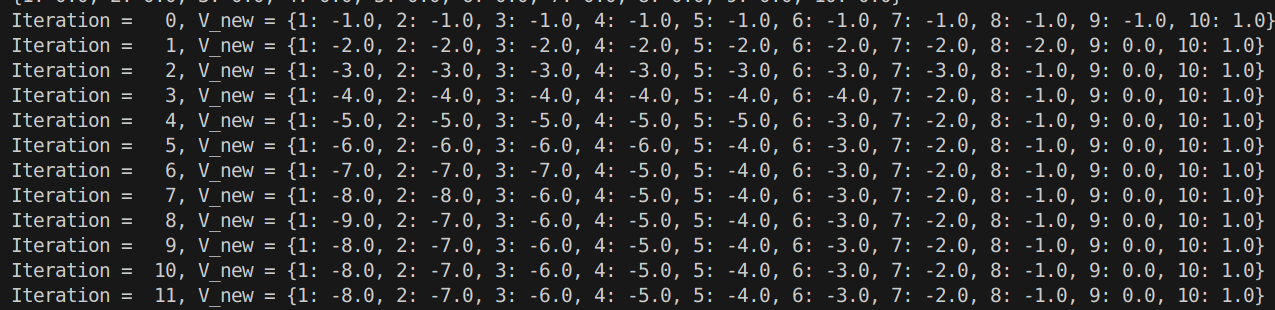
\includegraphics[width=\textwidth]{images/iters-of-value-iteration-1d-grid-world-code-output.png}
    \caption{Iterations of the value iteration algorithm.}
    \label{fig:iters-of-value-iteration-1d-grid-world-code-output}
\end{figure}


\section{Policy Iteration}


\section{Model-Free Learning Schemes}

Brilliant explanation in video 3 Mutual Information youtube video.  Key point is that $P(s',r|s,a)$ in Equation (\ref{eqn:action_value_function_definition}) is often unavailable in real-life practical problems and so we directly estimate the $q_*(s,a)$ by associating the final returns of episodic trajectories to state values (estimate $v(s)$) or state-action pairs (estimate $q(s,a)$).

\section{On-Policy and Off-Policy Learning}

For on-policy schemes the policy $\pi(s|a)$ is used to explore the state space:
\begin{equation} \label{eqn:on-policy-definition}
    \pi(a|s) = b(a|s)
\end{equation}
while for off-policy schemes e.g. Q-Learning, Off-Policy Monte Carlo etc. the roles are separated with exploration done by a separate behaviour policy, $b(a|s)$,:
\begin{equation} \label{eqn:off-policy-definition}
    \pi(a|s) \neq b(a|s)
\end{equation}

Since the sampling of trajectories is done using $b(a|s)$ instead of $\pi(a|s)$, importance sampling is used to rescale the sampled distributions to recover return contributions as if the sampled was done by $\pi(a|s)$.  This is similar to Umbrella Sampling in computational materials science.  One can initialise trajectories from any state and explore using the behaviour policy $b(a|s)$ and generate numerous trajectories and their associated returns.  Then use a credit assignment scheme like Monte Carlo Learning to assign values to either the state value function $v(s)$ of each state, or state-action values $q(s,a)$ to each state-action pair.










\end{document}


